\documentclass[unicode, notheorems]{beamer}

% If you have more than three sections or more than three subsections in at least one section,
% you might want to use the [compress] switch. In this case, only the current (sub-) section
% is displayed in the header and not the full overview.
\mode<presentation>
{
  \usetheme[numbers, totalnumbers, compress, nologo]{Statmod}

  \setbeamercovered{transparent}
  % or whatever (possibly just delete it)
}

%\usepackage{pscyr}
\usepackage[T2A]{fontenc}
\usepackage[utf8]{inputenc}
\usepackage[russian]{babel}
\usepackage{amsthm}
\usepackage{colortbl}
\usepackage{wrapfig}
\usepackage{tikz}
\usetikzlibrary{shapes, arrows}
\tikzstyle{decision} =
        [
                diamond,
                draw,
                fill = green!20,
                text width = 6em,
                text badly centered,
                node distance = 2cm,
                inner sep = 0pt
        ]
\tikzstyle{block} =
        [
                rectangle,
                draw,
                fill = blue!20,
                text width = 6em,
                text centered,
                rounded corners,
                minimum height = 2em
        ]
\tikzstyle{line} =
        [
                draw,
                -latex'
        ]
\tikzstyle{cloud} =
        [
                draw,
                ellipse,
                fill = red!20,
                node distance = 3cm,
                minimum height = 2em
        ]
% you only need this when using TikZ graphics

\newtheorem{theorem}{Theorem}
\newtheorem{example}{Example}
\newtheorem{definition}{Definition}

\title[Разработка тестового ПО для NetX 500]{Разработка тестового программного обеспечения для процессорных модулей на базе микропроцессора NetX~500}

\author{Смирнов В.Ю. А12-11}
\institute[НИЯУ МИФИ]{
\ \\
    Научный руководитель: ассистент каф. 27, Тихонов Ю.Н.\\
    Рецензент: ст. преп. каф. 26, Азаров Д.А.\\
    \vspace{1.6cm}
}
\date{
    НИЯУ МИФИ\\
    Москва\\
    2012 г.
}

\graphicspath{{images/}} % Где их искать

\subject{Beamer}
% This is only inserted into the PDF information catalog. Can be left
% out.

% Delete this, if you do not want the table of contents to pop up at
% the beginning of each subsection:
% \AtBeginSubsection[]
% {
%   \begin{frame}<beamer>
%     \frametitle{Outline}
%     \tableofcontents[currentsection,currentsubsection]
%   \end{frame}
% }

\begin{document}

\begin{frame}
    \titlepage
\end{frame}

\section{Введение}

\begin{frame}
    \frametitle{Цели проекта}
    \begin{itemize}
     \item Создание встраиваемого программного обеспечения для POST-тестирования процессорных модулей на базе NetX~500.
%     \item Создание встраиваемого программного обеспечения для производственного тестирования процессорных модулей на базе NetX~500.
     \item Разработка программного-аппаратного комплекса для тестирования и верификации модулей.
    \end{itemize}
\end{frame}

\begin{frame}
    \frametitle{Актуальность работы}
    \begin{itemize}
     \item Наличие потребности в системе контроля качества процессорных модулей
     \item Необходимость средства оперативной диагностики процессорных модулей непосредственно перед каждым включением
     \item Отсутствие широко распространенных реализаций систем производственного и POST-тестирования, рассчитанных на встраиваемые решения
    \end{itemize}
\end{frame}

\section{POST-тесты}

%\begin{frame}{Сервер автоматизации комплекса ТПТС-НТ}
%\end{frame}

\begin{frame}{Требования к POST-тестам}
\begin{figure}[h]
\begin{center}
	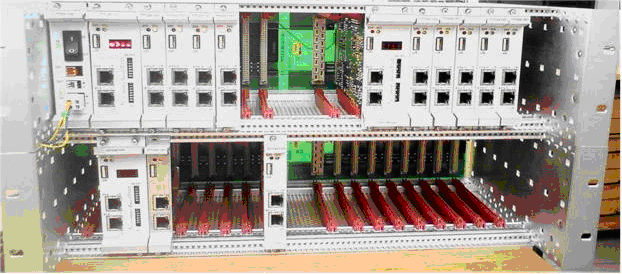
\includegraphics[width=0.8\columnwidth]{AS}
\end{center}
\end{figure}
\begin{itemize}
 \item Выполнение при каждом старте
 \item Время выполнения менее 1 секунды
 \item Тестовое воздействие не должно выходить за пределы модуля
 \item Выполнение автоматизировано
 \item При ошибке -- прервать загрузку
\end{itemize}
\end{frame}

\begin{frame}{Реализация POST-тестов}
\begin{columns}[c]
\begin{column}{0.5\linewidth}
\begin{itemize}
 \item Основной язык: C
 \item Более 2000 строк кода:
 \begin{itemize}
  \item 1300 -- драйвера
  \item 700 -- тесты
 \end{itemize}

 \item Проводят тестирование:
 \begin{itemize}
  \item SRAM
  \item SDRAM
  \item SPI Flash
  \item LED
  \item Profibus
 \end{itemize}
\end{itemize}

\end{column}
\begin{column}{0.5\linewidth}
\begin{figure}[h]
\begin{center}
\tikzset{
	every node/.style={scale=0.75}
}
\begin{tikzpicture}[node distance = 1.25cm, auto]
        \node [cloud] (start) {Начало};
        \node [block, below of = start, node distance = 2cm] (phase1) {Запуск тестов};
%        \node [block, below of = phase1] (phase2) {Этап 2};
%        \node [block, below of = phase2] (phase3) {Этап 3};
%        \node [block, below of = phase3] (phase4) {Этап 4};
%        \node [block, below of = phase4] (phase5) {Этап 5};
%        \node [block, below of = phase5] (phase6) {Этап 6};
%        \node [block, below of = phase1] (phase7) {Этап 7};
%        \node [block, left of = phase1, node distance = 3cm] (correction) {Коррекция};
        \node [decision, below of = phase1, node distance = 2.5cm] (condition) {Ошибка?};
        \node [block, below of = condition, node distance = 2.5cm] (finish) {Загрузка ВПО};
	\node [block, left of = finish, node distance = 3cm] (failish) {Прерывание\\работы};

        \path [line] (start) -- (phase1);
%        \path [line] (phase1) -- (phase2);
%        \path [line] (phase2) -- (phase3);
%        \path [line] (phase3) -- (phase4);
%        \path [line] (phase4) -- (phase5);
%        \path [line] (phase5) -- (phase6);
%        \path [line] (phase6) -- (phase7);
        \path [line] (phase1) -- (condition);
        \path [line] (condition) -| node [near start] {Да} (failish);
%        \path [line] (correction) |- (phase1);
        \path [line] (condition) -- node {Нет}(finish);
\end{tikzpicture}
%	\includegraphics[width=1.0\columnwidth]{stend}
\end{center}
\end{figure}
\end{column}
\end{columns}
\end{frame}

\section{Производственные тесты}
\begin{frame}{Схема тестового стенда}
\begin{columns}[c]

\begin{column}{0.4\linewidth}
\begin{itemize}
 \item Крейт
 \item ПК
 \item Тестируемые модули
\end{itemize}

\end{column}
\begin{column}{0.75\linewidth}
\begin{figure}[h]
\begin{center}
	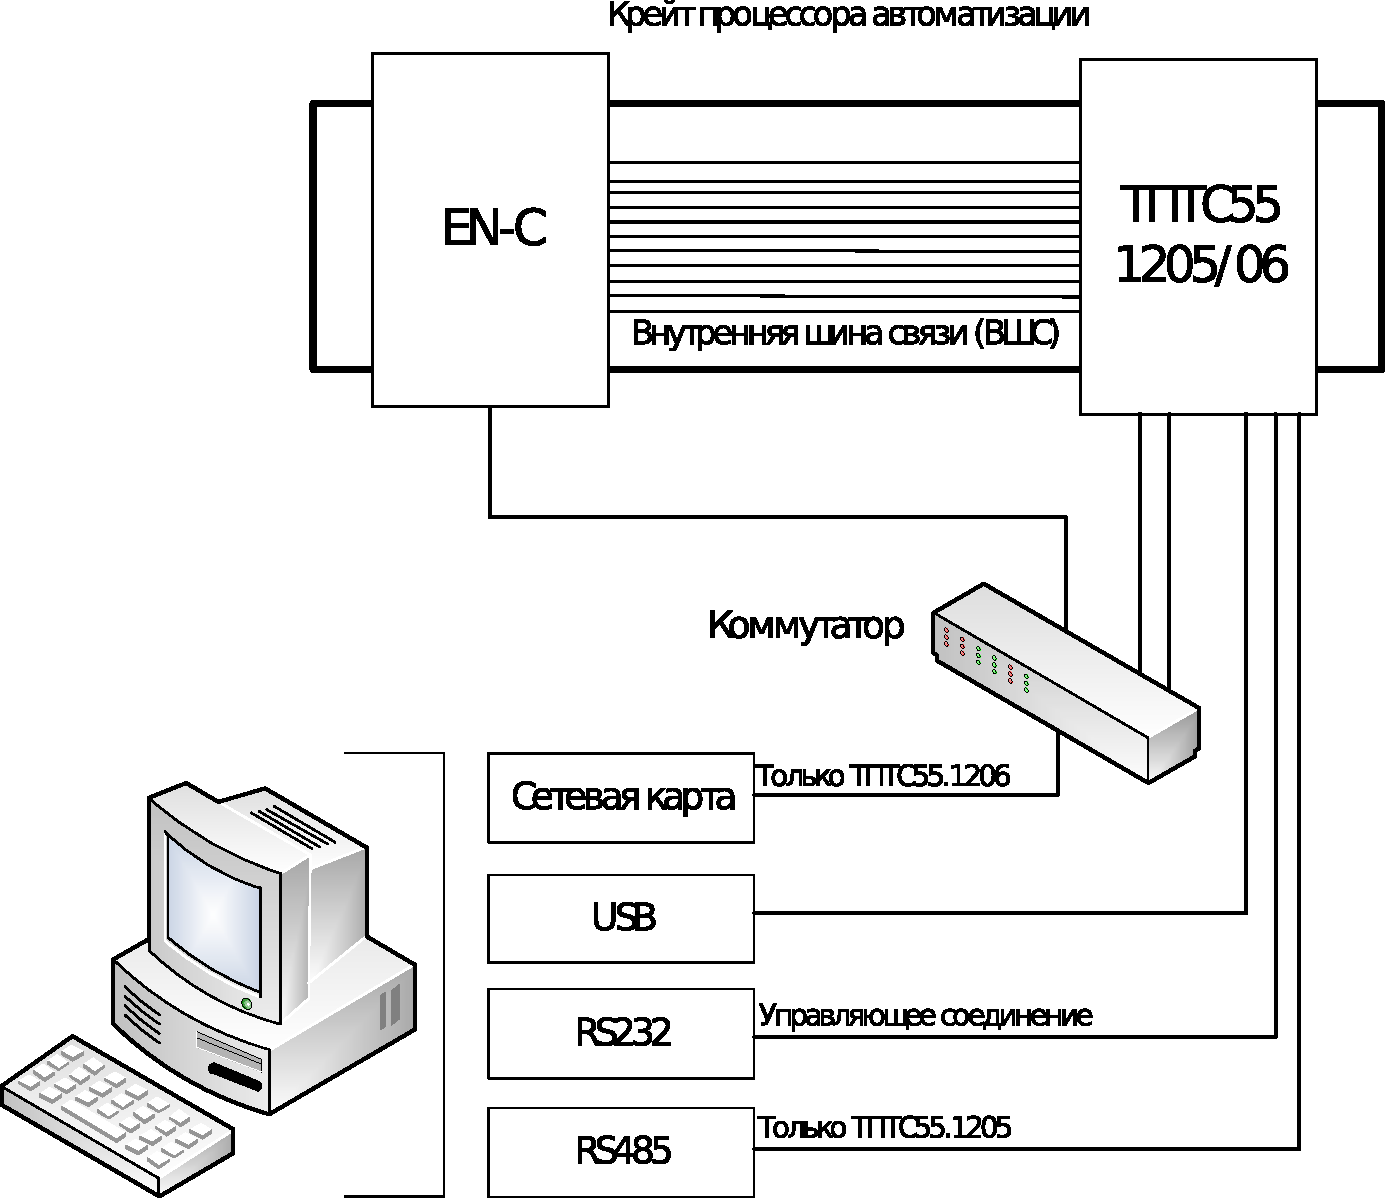
\includegraphics[width=1.0\columnwidth]{test-stend}
\end{center}
\end{figure}
\end{column}
\end{columns}
\end{frame}

\begin{frame}{Требования к производственным тестам}
 \begin{columns}[c]
  \begin{column}{0.6\linewidth}
   \begin{figure}[h]
    \begin{center}
      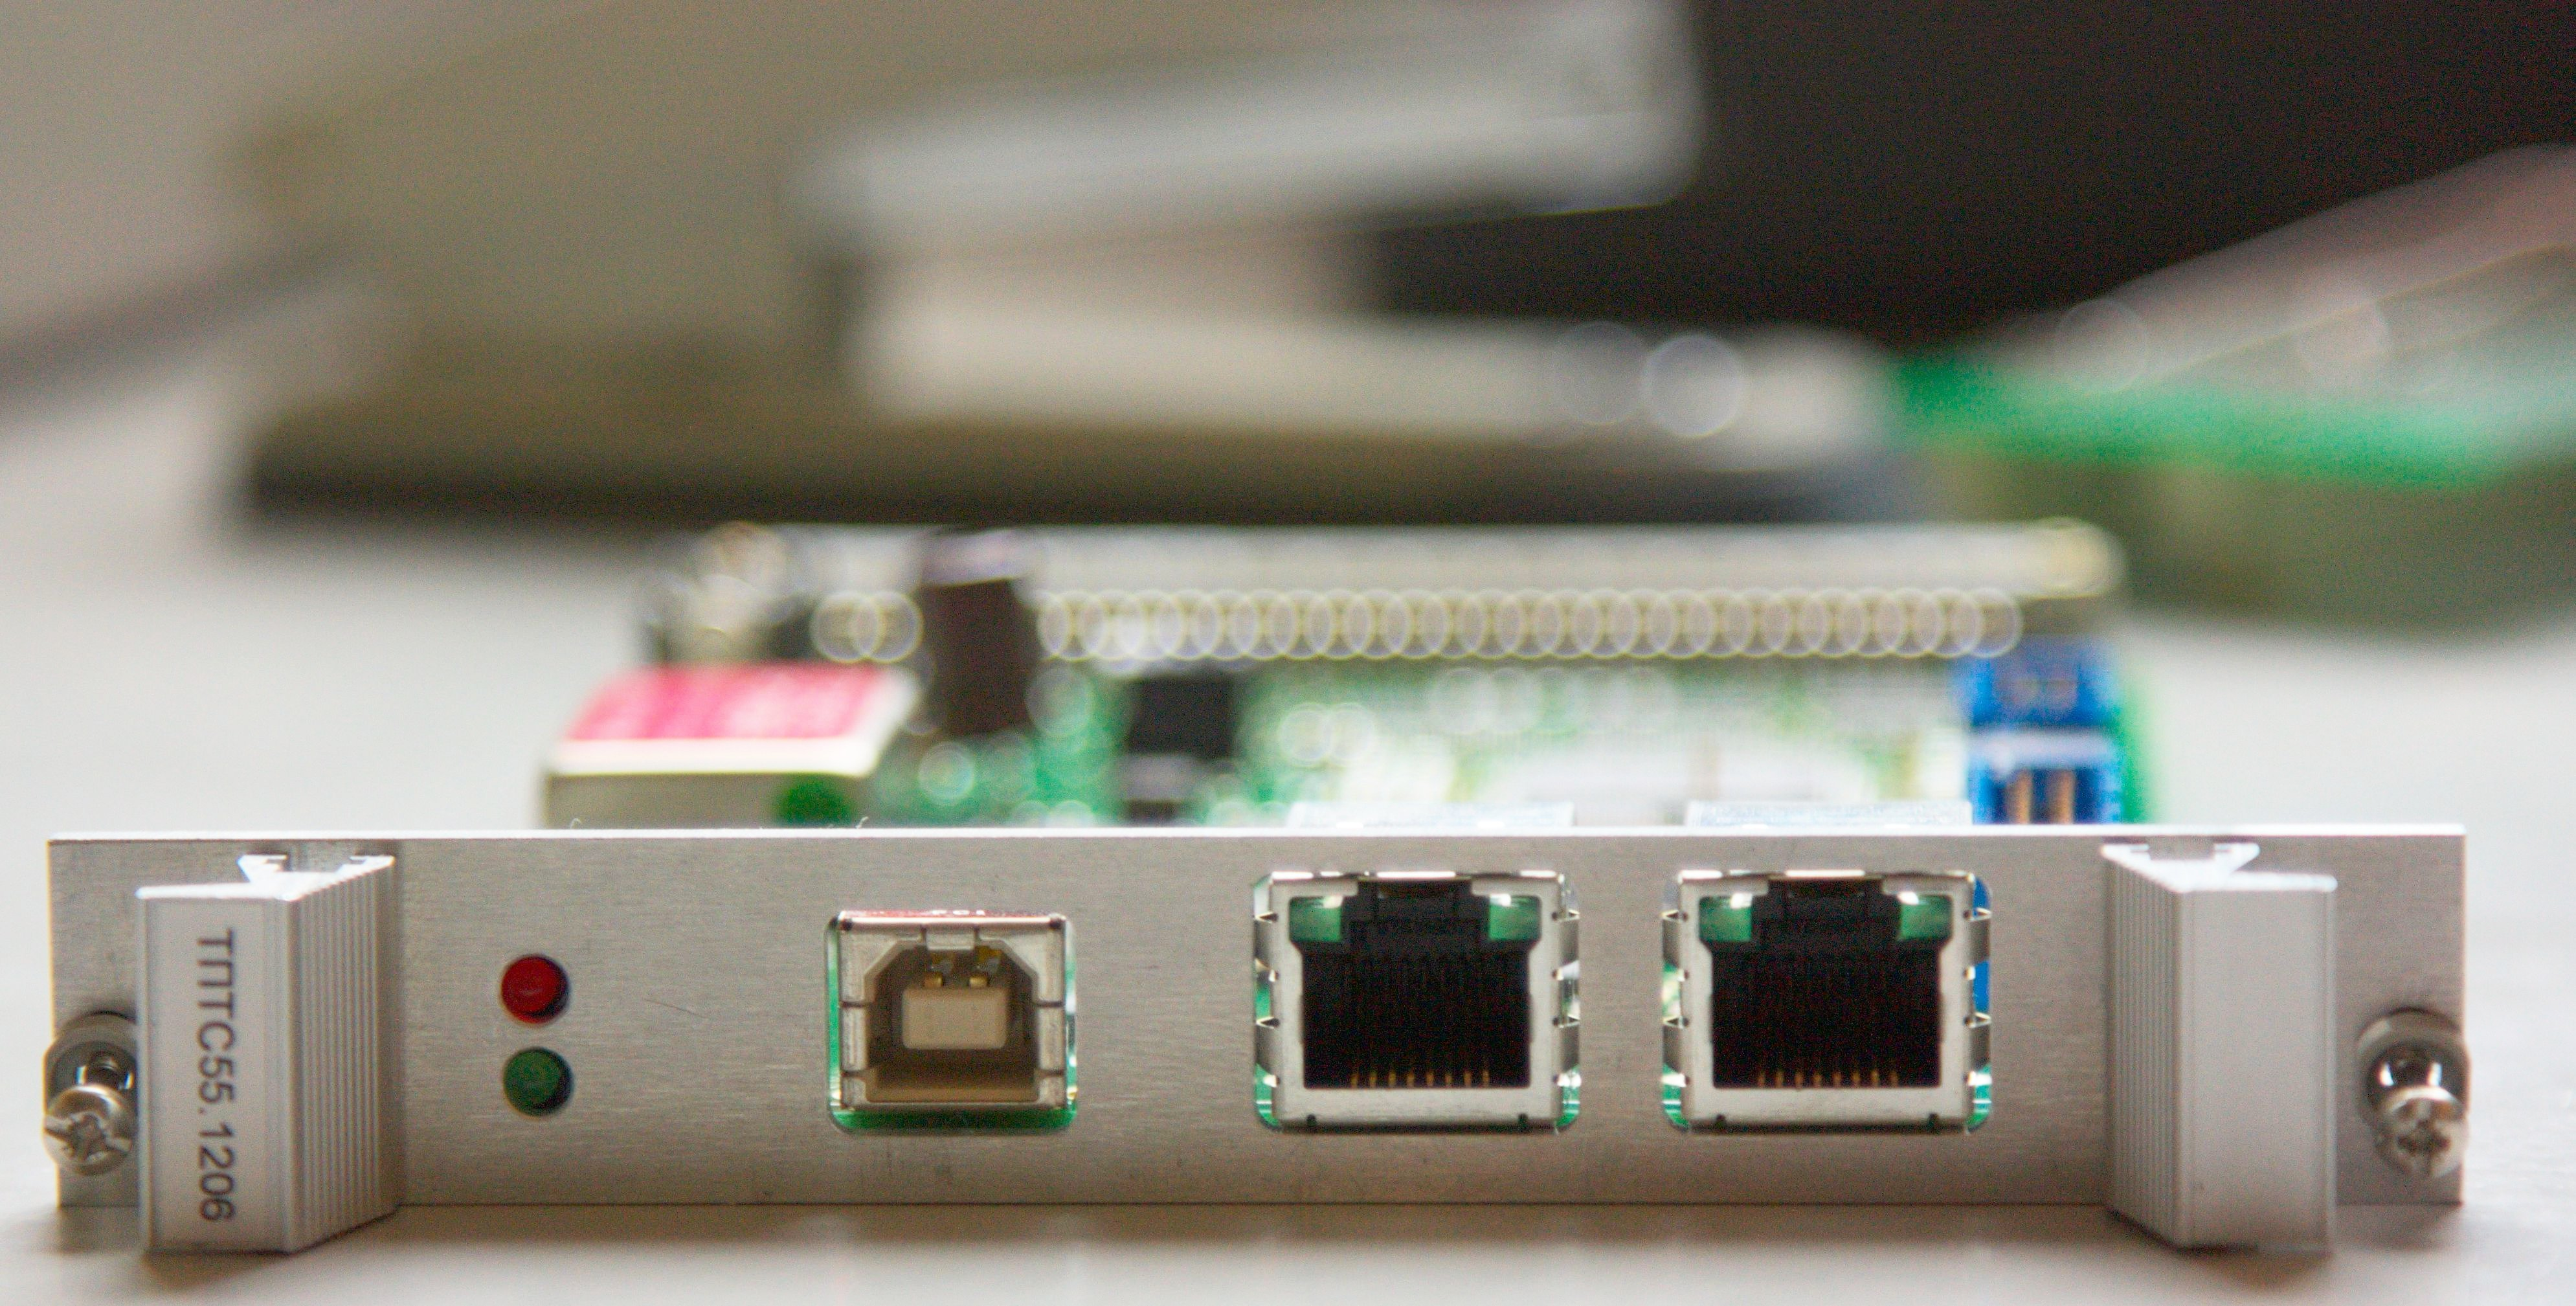
\includegraphics[width=1.0\columnwidth]{tpts_1206}
    \end{center}
   \end{figure}
  \end{column}
  \begin{column}{0.5\linewidth}
   \begin{figure}[h]
    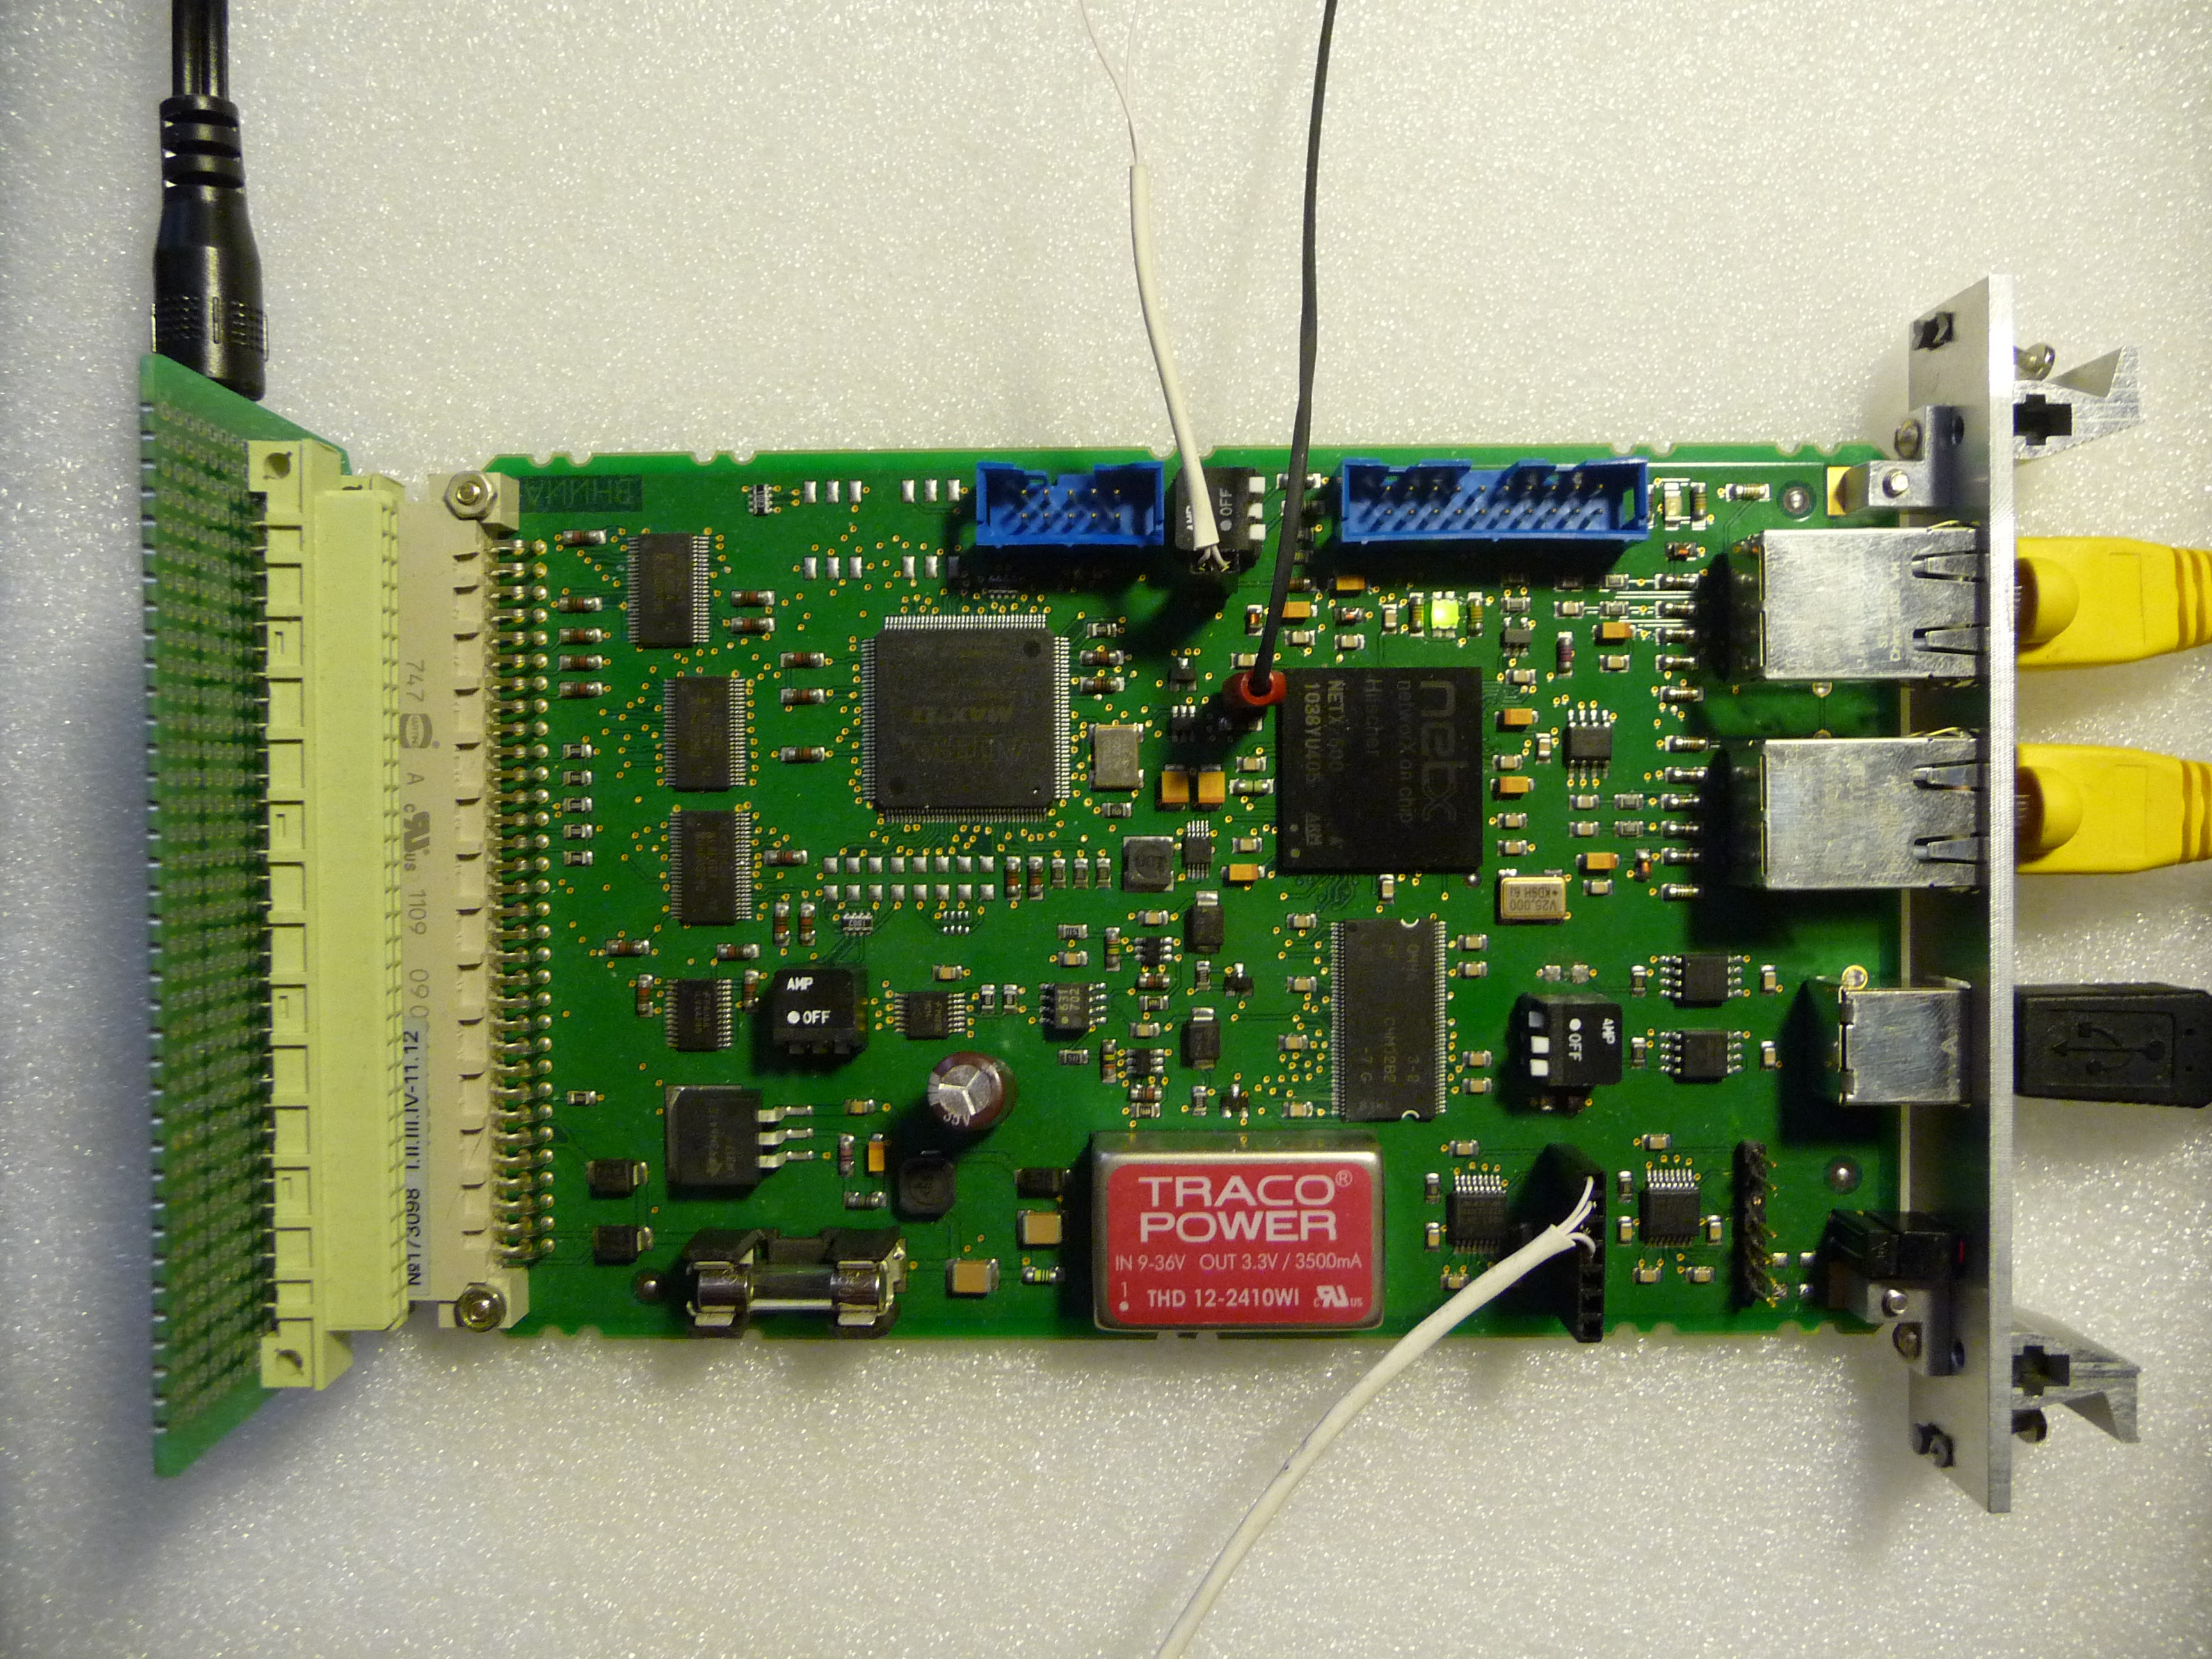
\includegraphics[width=0.81\columnwidth]{P1030165}
   \end{figure}
  \end{column}
 \end{columns}
 \begin{itemize}
  \item Исполняются в диагностическом режиме
  \item Время выполнения не ограничено
  \item Проверка происходит при участии оператора
  \item Возможность автоматизировать исполнение тестов на объекте при помощью скриптов
 \end{itemize}
\end{frame}

\begin{frame}{Реализация производственных тестов}
\begin{columns}[c]
\begin{column}{0.44\linewidth}
\begin{itemize}
 \item Основной язык: C
 \item Более 7000 строк кода:
  \begin{itemize}
   \item 6000 -- драйвера
   \item 1000 -- тесты
  \end{itemize}
 \item Проводит тестирование:
 \begin{itemize}
  \item SDRAM, SRAM
  \item USB, Ethernet, Profibus
  \item LED, GPIO
  \item SPI Flash
 \end{itemize}
\end{itemize}
\end{column}
\begin{column}{0.56\linewidth}
\begin{figure}[h]
\begin{center}
\tikzset{
	every node/.style={scale=0.5}
}
\begin{tikzpicture}[node distance = 2cm, auto]
        \node [cloud] (start) {Начало};
        \node [block, below of = start] (phase1) {Инициали\-зация};
        \node [block, below of = phase1, node distance = 2cm] (phase2) {Ожидание команды};
	\node [decision, below of = phase2, node distance = 3cm] (cond1) {Какая команда?};
	\node [block, left of = cond1, node distance = 5cm] (unk) {Ошибка};
	\node [block, right of = cond1, node distance = 5cm] (ping) {Ответ};
	\node [block, below of = cond1, node distance = 3cm] (phase3) {Выполнение теста};
	\node [cloud, below of = phase3, node distance = 2cm] (finish) {Перезагрузка};


        \path [line] (start) -- (phase1);
        \path [line] (phase1) -- (phase2);
        \path [line] (phase2) -- (cond1);
	\path [line] (cond1) -- node {ping} (ping);
	\path [line] (cond1) -- node {неизв.} (unk);
	\path [line] (cond1) -- node {run} (phase3);
	\path [line] (phase3) -- (finish);
	\path [line] (unk) |- (phase2);
	\path [line] (ping) |- (phase2);

%        \path [line] (phase3) -- (phase4);
%        \path [line] (phase4) -- (phase5);
%        \path [line] (phase5) -- (phase6);
%        \path [line] (phase6) -- (phase7);
%        \path [line] (phase1) -- (condition);
%        \path [line] (condition) -| node [near start] {Да} (failish);
%        \path [line] (correction) |- (phase1);
%        \path [line] (condition) -- node {Нет}(finish);

	
%        \node [block, below of = phase2] (phase3) {Выполнение теста};
%        \node [block, below of = phase3] (phase4) {Этап 4};
%        \node [block, below of = phase4] (phase5) {Этап 5};
%        \node [block, below of = phase5] (phase6) {Этап 6};
%        \node [block, below of = phase1] (phase7) {Этап 7};
%        \node [block, left of = phase1, node distance = 3cm] (correction) {Коррекция};
%        \node [decision, below of = phase1] (condition) {Ошибка?};
%        \node [cloud, below of = condition] (finish) {Загрузка ВПО};
%        \node [cloud, left of = finish, node distance = 3.5cm] (failish) {Ошибка};

%        \path [line] (start) -- (phase1);
%        \path [line] (phase1) -- (phase2);
%        \path [line] (phase2) -- (phase3);
%        \path [line] (phase3) -- (phase4);
%        \path [line] (phase4) -- (phase5);
%        \path [line] (phase5) -- (phase6);
%        \path [line] (phase6) -- (phase7);
%        \path [line] (phase1) -- (condition);
%        \path [line] (condition) -| node [near start] {Да} (failish);
%        \path [line] (correction) |- (phase1);
%        \path [line] (condition) -- node {Нет}(finish);
\end{tikzpicture}
%	\includegraphics[width=1.0\columnwidth]{stend}
\end{center}
\end{figure}
\end{column}
\end{columns}
\end{frame}

\begin{frame}{Интерфейс прикладного ПО для проведения производственного тестирования}
%\begin{figure}[h]
%\begin{center}
%	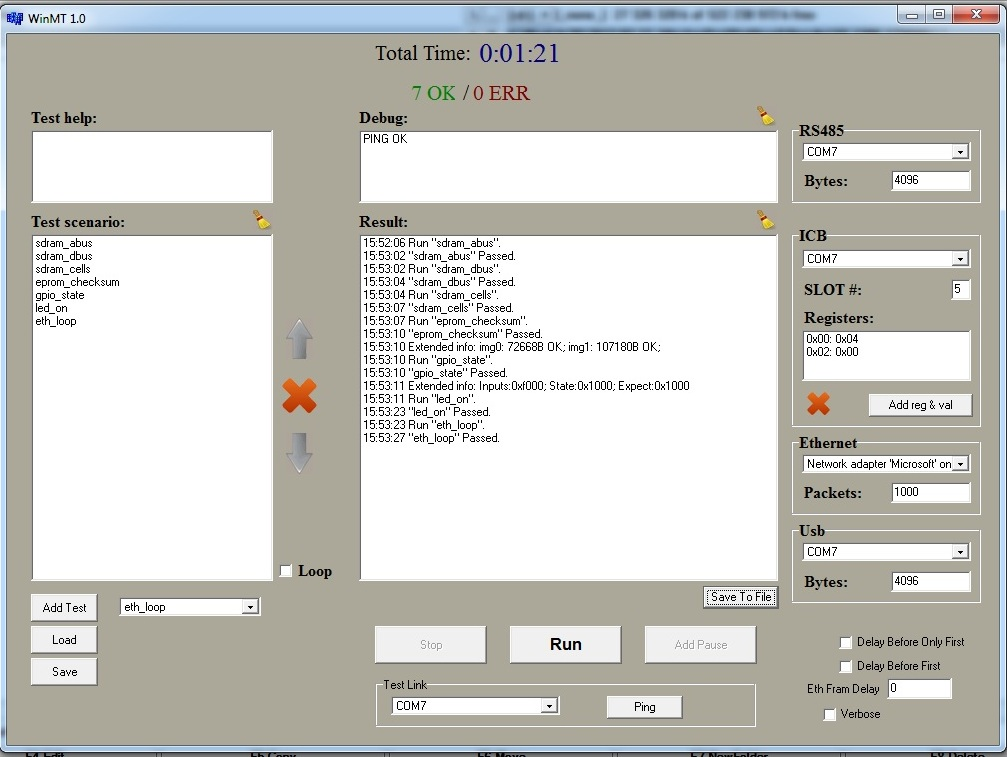
\includegraphics[width=0.8\columnwidth]{1206-ok}
%\end{center}
%\end{figure}
%\end{frame}
%\begin{frame}{Реализация}
\begin{columns}[c]
\begin{column}{0.45\linewidth}
\begin{itemize}
 \item Основной язык: C++
 \item Более 6000 строк кода
\end{itemize}
\end{column}
\begin{column}{0.63\linewidth}
\begin{figure}[h]
\begin{center}
	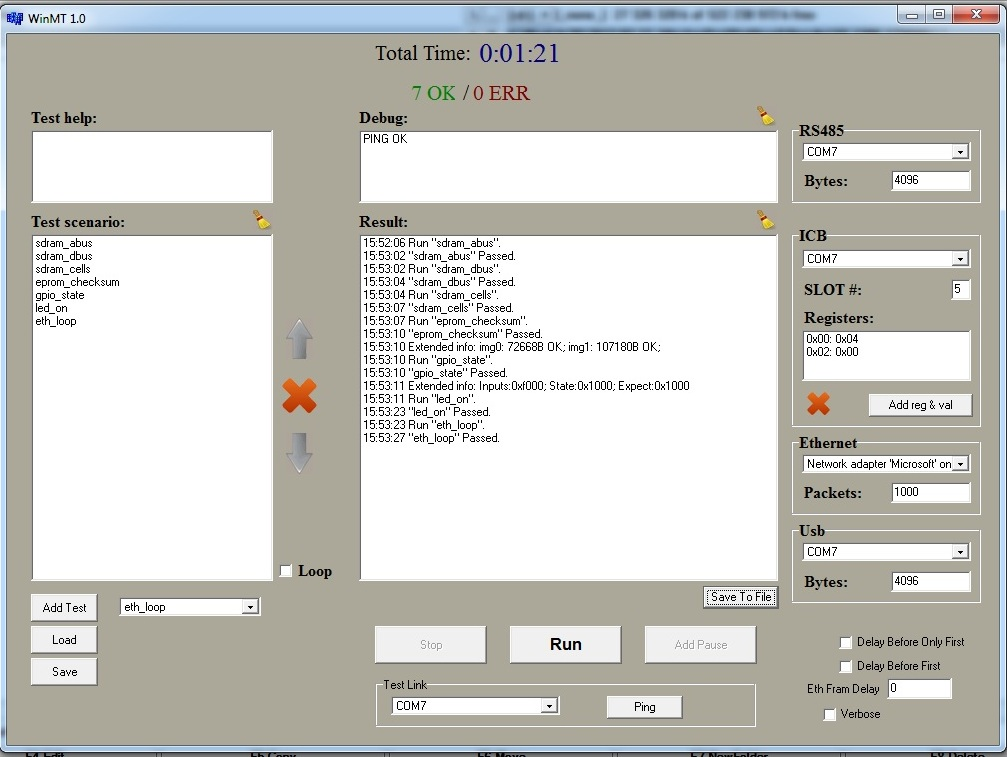
\includegraphics[width=1.0\columnwidth]{1206-ok}
\end{center}
\end{figure}
\end{column}
\end{columns}
\end{frame}

\section{Архитектурные решения}
\begin{frame}{Особенности системы тестирования}
 \begin{itemize}
 \item POST и производственные тесты располагаются в различных микросхемах SPI Flash
 \item В случае ошибки POST загрузка ВПО не выполнятся
 \item Тесты POST не выполняются при запуске MT-тестов
 \item Возможность загрузки нескольких образов ВПО
 \item Две системы сборки -- HiTOP и GNU Make
\end{itemize}
\end{frame}

\section{Результаты}
\begin{frame}{Результаты тестирования}
\begin{center}
\begin{tabular}{|c|c|c|c|}
\hline Тест & ТПТС55.1206 & ТПТС55.1205 & Плата развития \\\hline
EPROM & \textcolor[rgb]{0,0.5,0}{\textbf{\texttt{+}}} &\textcolor[rgb]{0,0.5,0}{\textbf{\texttt{+}}}&\textcolor[rgb]{0,0.5,0}{\textbf{\texttt{+}}}\\\hline
Ethernet &\textcolor[rgb]{0,0.5,0}{\textbf{\texttt{+}}}& N/A &\textcolor[rgb]{0,0.5,0}{\textbf{\texttt{+}}}\\\hline
FPGA & \textcolor{red}{\textbf{\texttt{-}}} & \textcolor{red}{\textbf{\texttt{-}}} & N/A \\\hline
GPIO &\textcolor[rgb]{0,0.5,0}{\textbf{\texttt{+}}}&\textcolor[rgb]{0,0.5,0}{\textbf{\texttt{+}}}&\textcolor[rgb]{0,0.5,0}{\textbf{\texttt{+}}}\\\hline
DPRAM & \textcolor{red}{\textbf{\texttt{-}}} & \textcolor{red}{\textbf{\texttt{-}}} & N/A \\\hline
LED &\textcolor[rgb]{0,0.5,0}{\textbf{\texttt{+}}}&\textcolor[rgb]{0,0.5,0}{\textbf{\texttt{+}}}&\textcolor[rgb]{0,0.5,0}{\textbf{\texttt{+}}}\\\hline
RS485 & N/A &\textcolor[rgb]{0,0.5,0}{\textbf{\texttt{+}}}&\textcolor[rgb]{0,0.5,0}{\textbf{\texttt{+}}}\\\hline
SDRAM &\textcolor[rgb]{0,0.5,0}{\textbf{\texttt{+}}}&\textcolor[rgb]{0,0.5,0}{\textbf{\texttt{+}}}&\textcolor[rgb]{0,0.5,0}{\textbf{\texttt{+}}}\\\hline
USB &\textcolor[rgb]{0,0.5,0}{\textbf{\texttt{+}}}&\textcolor[rgb]{0,0.5,0}{\textbf{\texttt{+}}}&\textcolor[rgb]{0,0.5,0}{\textbf{\texttt{+}}}\\\hline
\end{tabular}
\end{center}
\end{frame}

%TODO: Добавить список тестов, информацию по количеству строк, объему кода и т.п. Мб касивые схемы.
% Объединить второй и третий пункт во введении.
% Переформулировать в POST-тесха почему они не должны ни на кого воздействовать.
% Процент охвата тестами

\section{Заключение}

\begin{frame}
  \frametitle{Выводы}

  \begin{itemize}
   \item Разработанный тестовый комплекс позволяет проводить контроль качества процессорных модулей на всех этапах эксплуатации
   \item Разработанный комплекс POST-тестов позволяет проводить процедуры самопроверки в процессе нормальной эксплуатации модулей
   \item Тестирования первой партии образцов обнаружило и подтвердило неработоспособность некоторых коммуникационных интерфейсов полученных процессорных модулей
  \end{itemize}

\end{frame}

\begin{frame}
\begin{block}{}
        \center\LARGEСпасибо за внимание!
\end{block}
\end{frame}

\end{document}
